\chapter{Complementos del SGDWP}\label{anx:sgdwp}  % MARK: Complementos del SGDWP

\section{Iteraciones Adicionales}\label{sec:sgdwp-iteraciones-adicionales}  % MARK: - Iteraciones Adicionales

A continuación se presentan las primeras y últimas iteraciones que pasaron los baricentros proyectados de la Sección~\ref{sec:sgdwp}. En particular, los baricentros de las Figuras~\ref{fig:bar-SGDWP-pe}.
Recordar que en este caso se utilizó los parámetros $n_P\in\left\{ 1, 3, 5, 10 \right\}$.

\begin{figure}[htbp]
    \centering
    \begin{subfigure}[b]{0.8\textwidth}
        \centering
        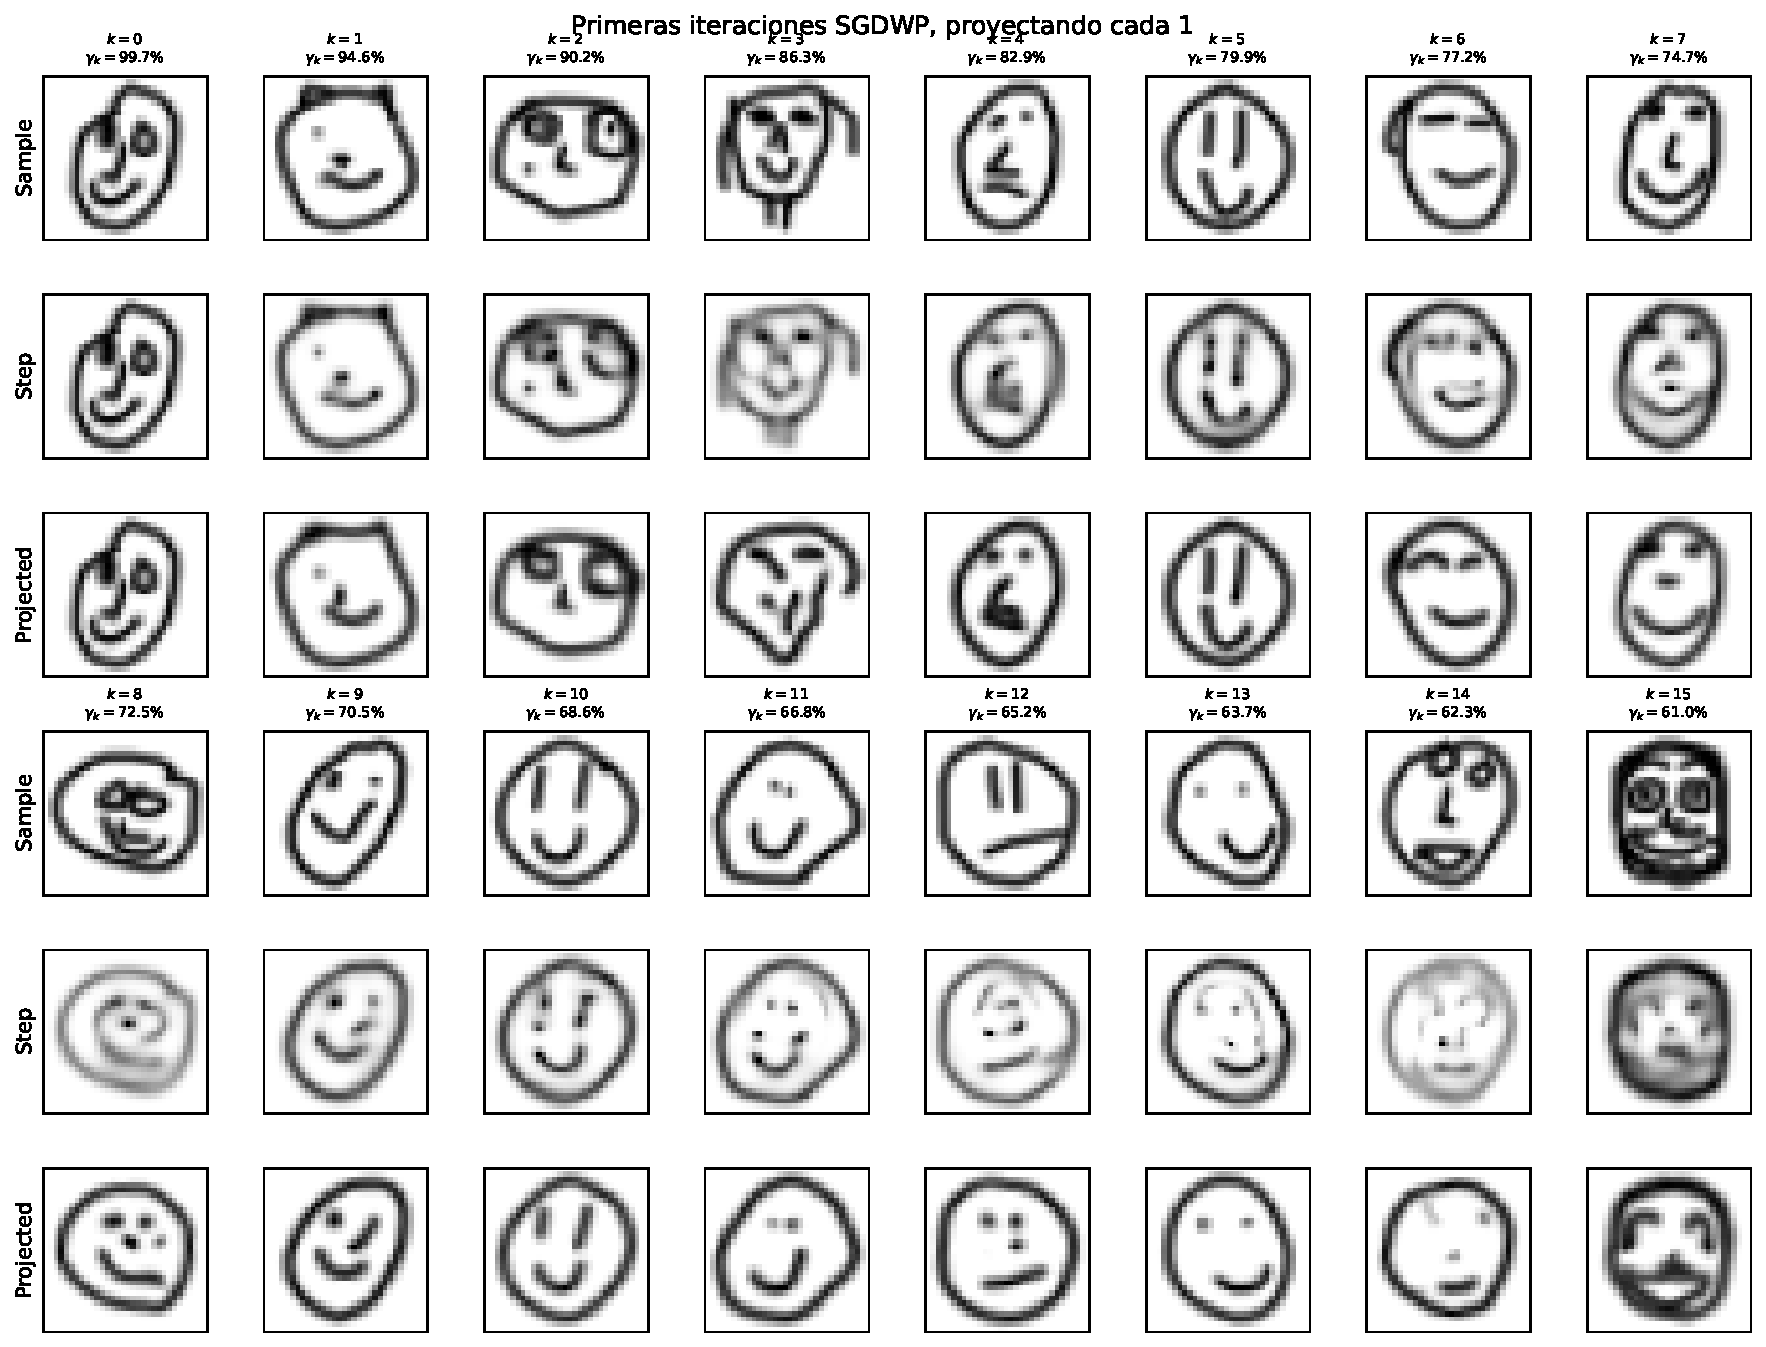
\includegraphics[width=\textwidth]{img/sgdwp-pe-iters/first-iters-pe-01.pdf}
        \caption{Primeras iteraciones del baricentro de la Fig.~\ref{fig:bar-SGDWP-pe-01}}
        \label{fig:first-iters-pe-01}
    \end{subfigure}
    \begin{subfigure}[b]{0.8\textwidth}
        \centering
        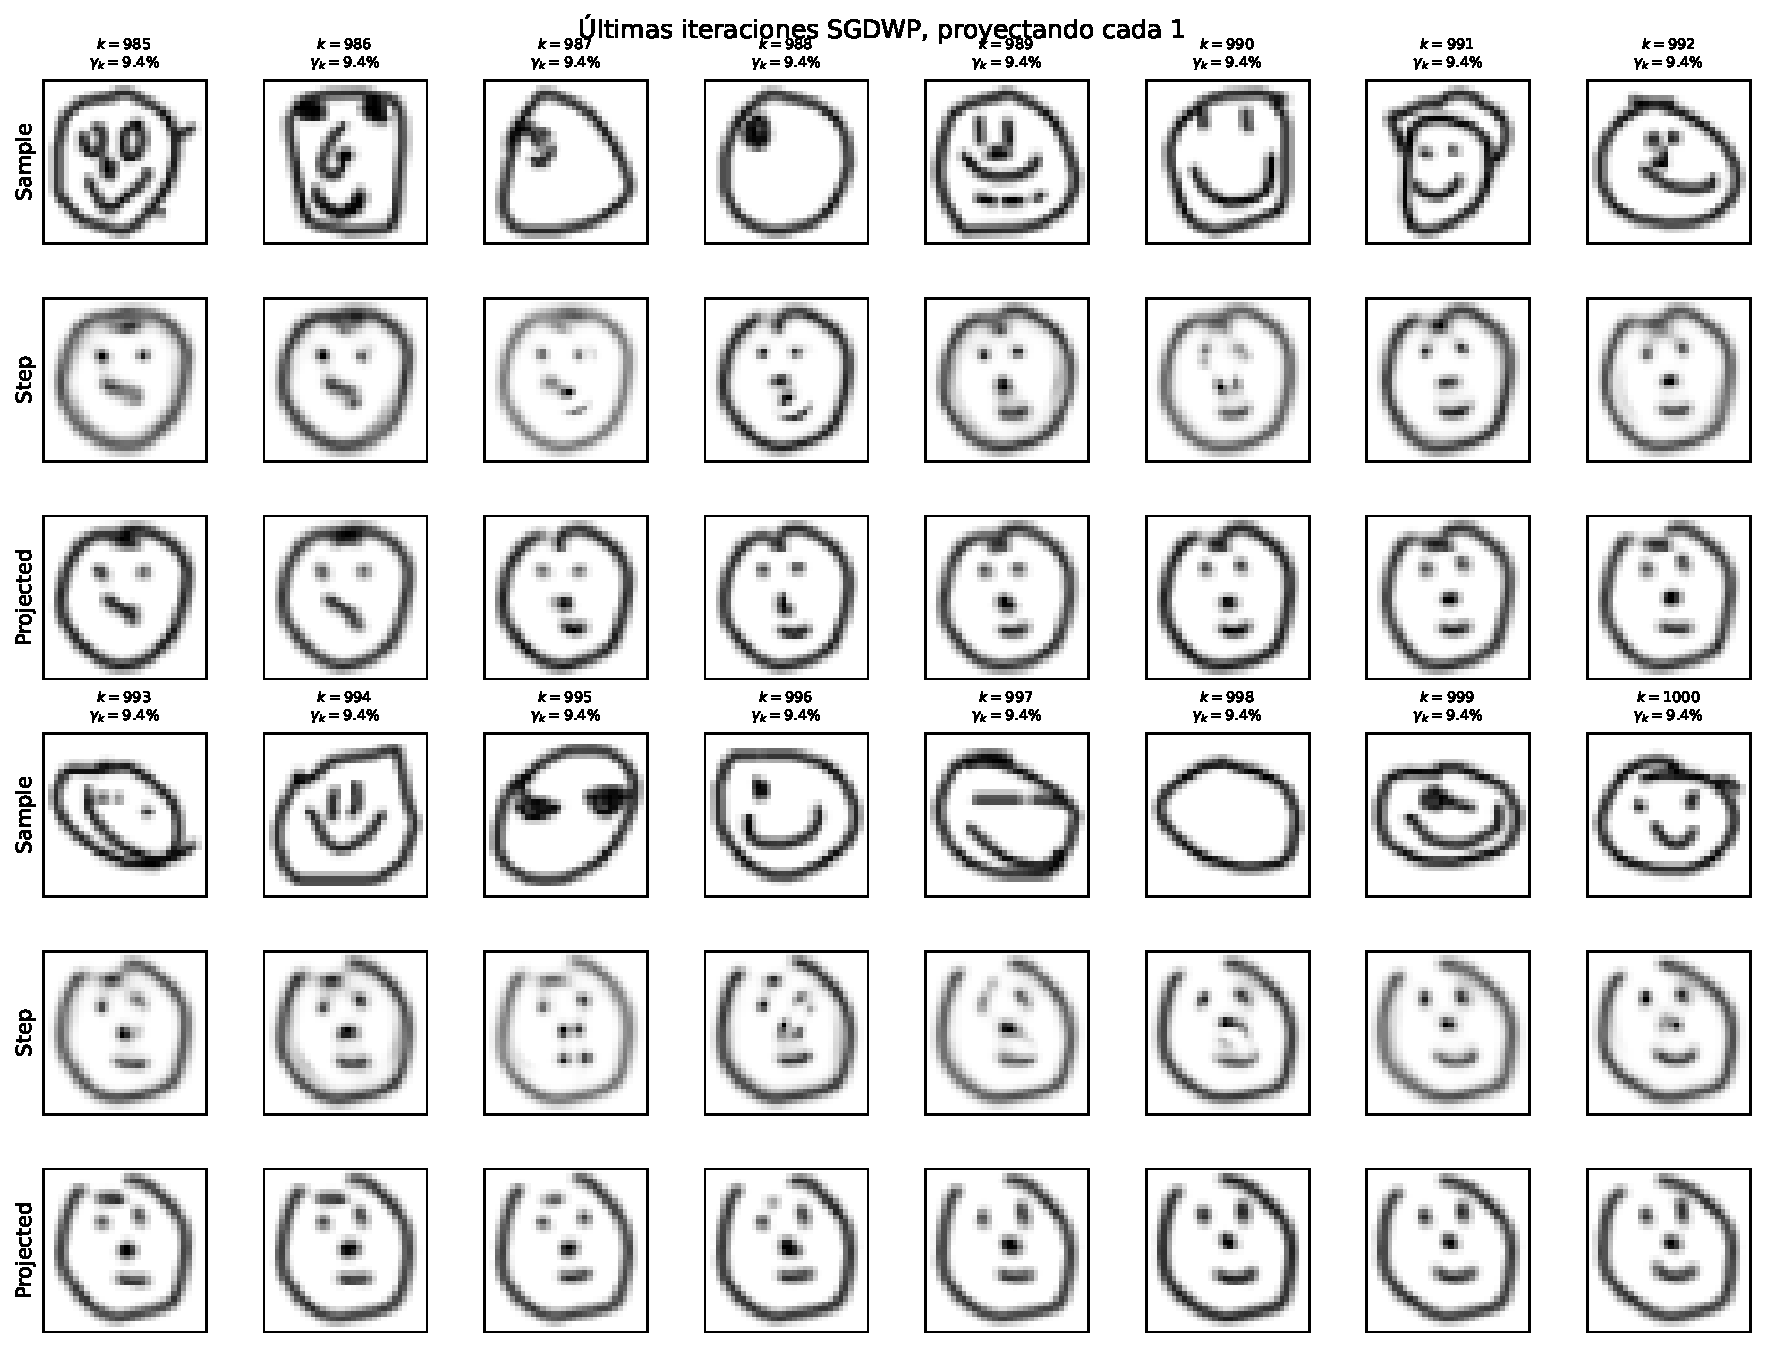
\includegraphics[width=\textwidth]{img/sgdwp-pe-iters/last-iters-pe-01.pdf}
        \caption{Últimas iteraciones del baricentro de la Fig.~\ref{fig:bar-SGDWP-pe-01}}
        \label{fig:last-iters-pe-01}
    \end{subfigure}
    \caption{Iteraciones del cálculo del baricentro de la Fig.~\ref{fig:bar-SGDWP-pe-01}.}
    \label{fig:iters-pe-01}
\end{figure}

\begin{figure}[htbp]
    \centering
    \begin{subfigure}[b]{0.8\textwidth}
        \centering
        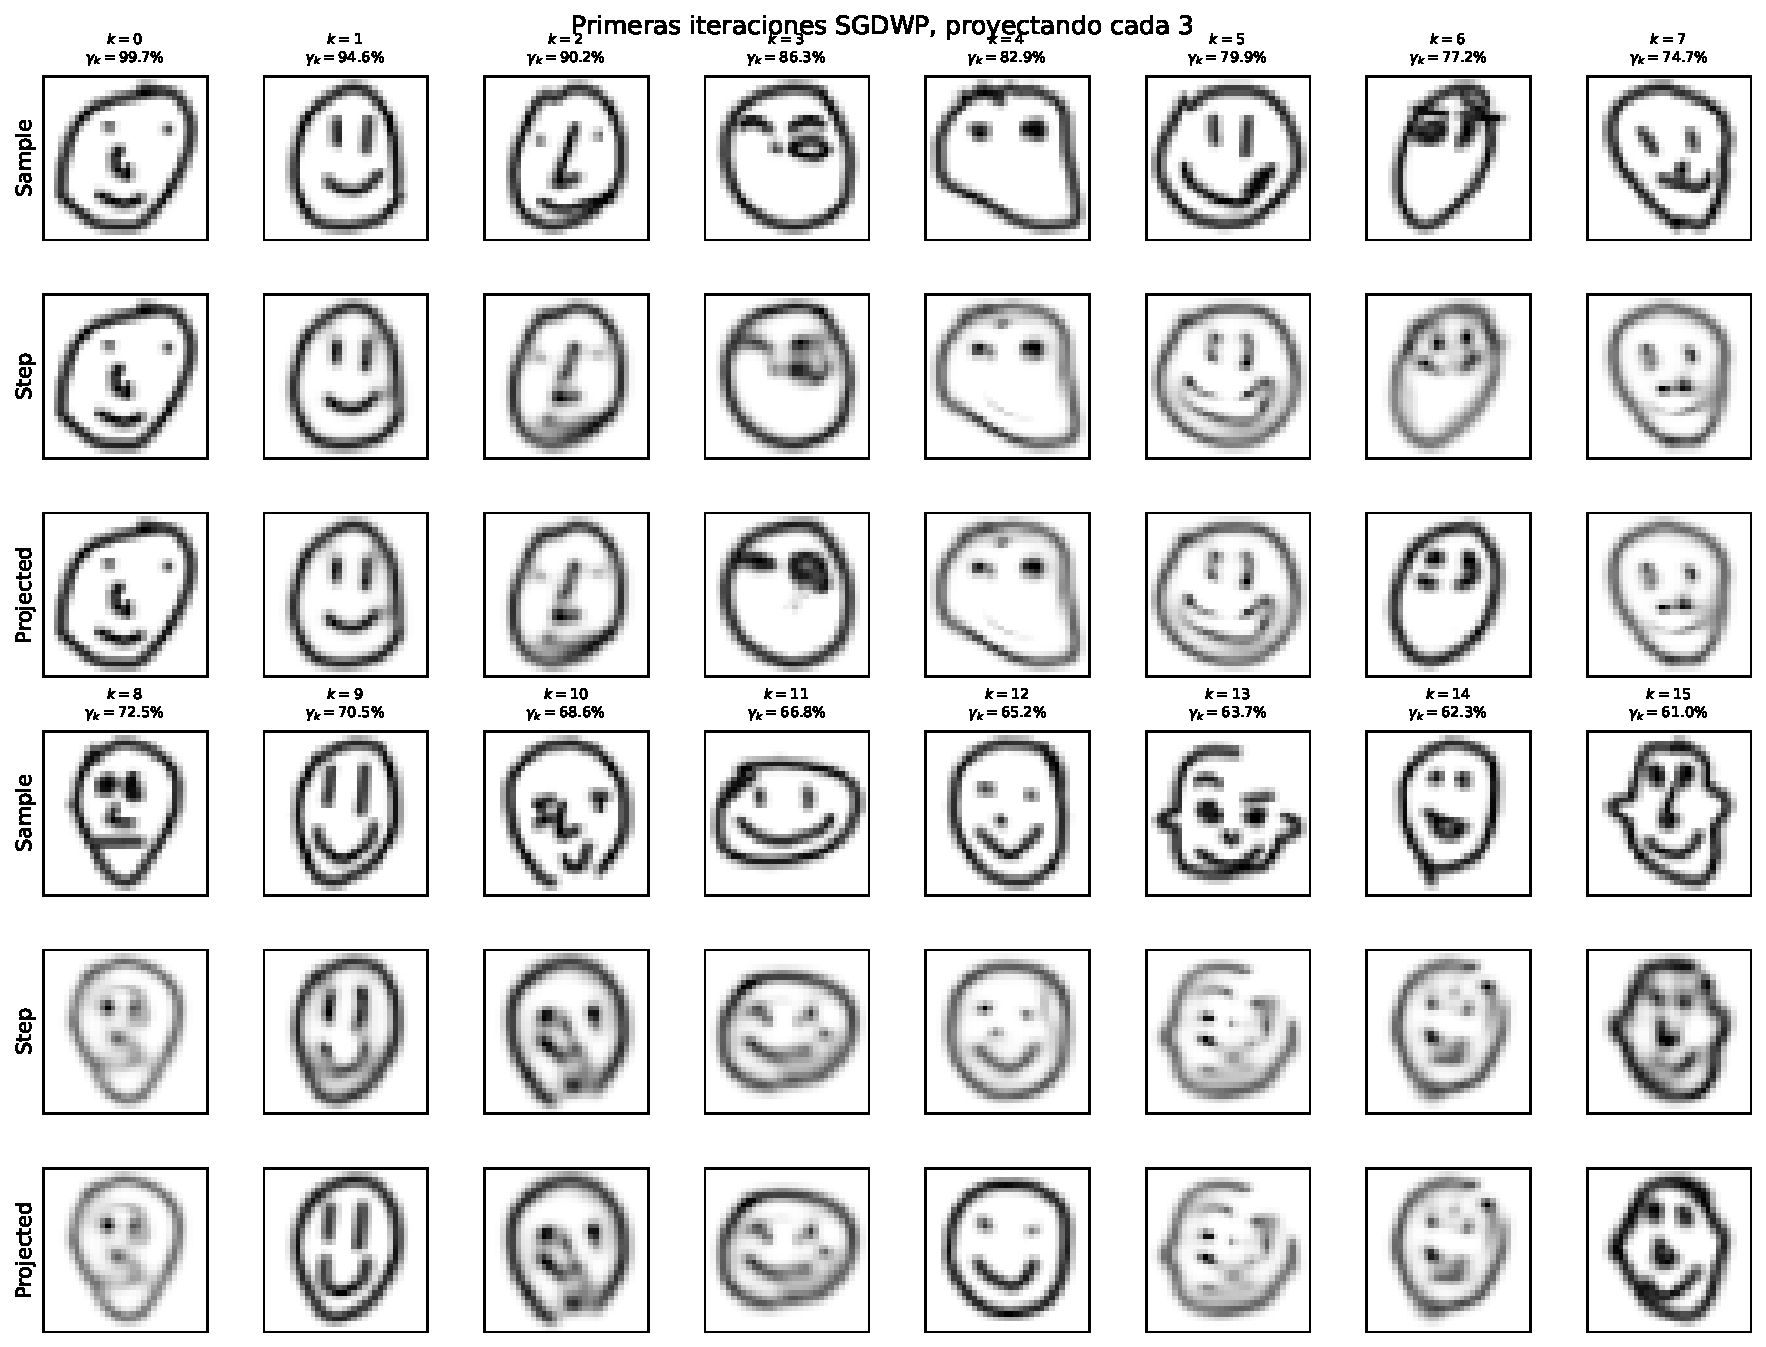
\includegraphics[width=\textwidth]{img/sgdwp-pe-iters/first-iters-pe-03.pdf}
        \caption{Primeras iteraciones del baricentro de la Fig.~\ref{fig:bar-SGDWP-pe-03}}
        \label{fig:first-iters-pe-03}
    \end{subfigure}
    \begin{subfigure}[b]{0.8\textwidth}
        \centering
        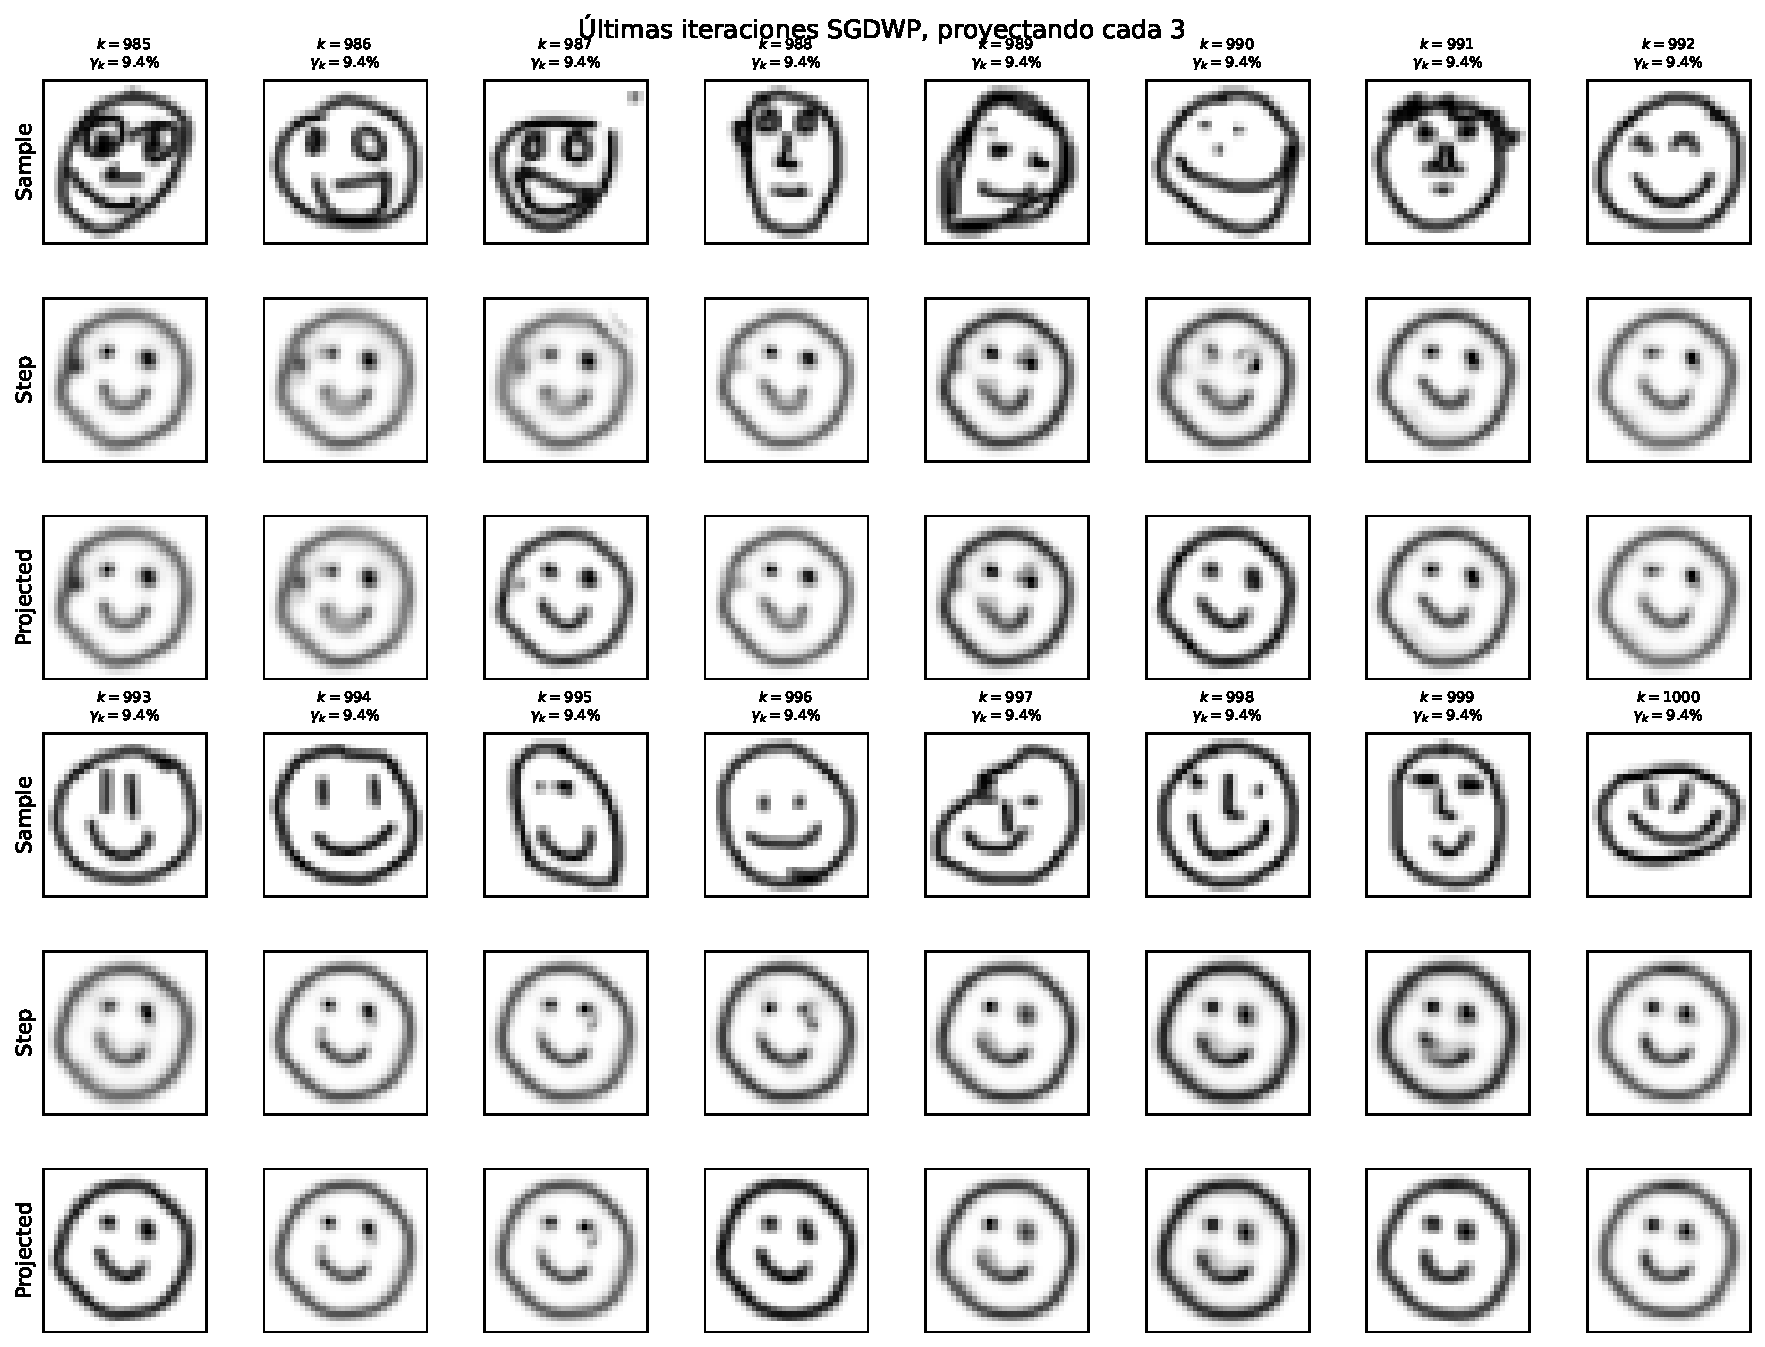
\includegraphics[width=\textwidth]{img/sgdwp-pe-iters/last-iters-pe-03.pdf}
        \caption{Últimas iteraciones del baricentro de la Fig.~\ref{fig:bar-SGDWP-pe-03}}
        \label{fig:last-iters-pe-03}
    \end{subfigure}
    \caption{Iteraciones del cálculo del baricentro de la Fig.~\ref{fig:bar-SGDWP-pe-03}.}
    \label{fig:iters-pe-03}
\end{figure}

\begin{figure}[htbp]
    \centering
    \begin{subfigure}[b]{0.8\textwidth}
        \centering
        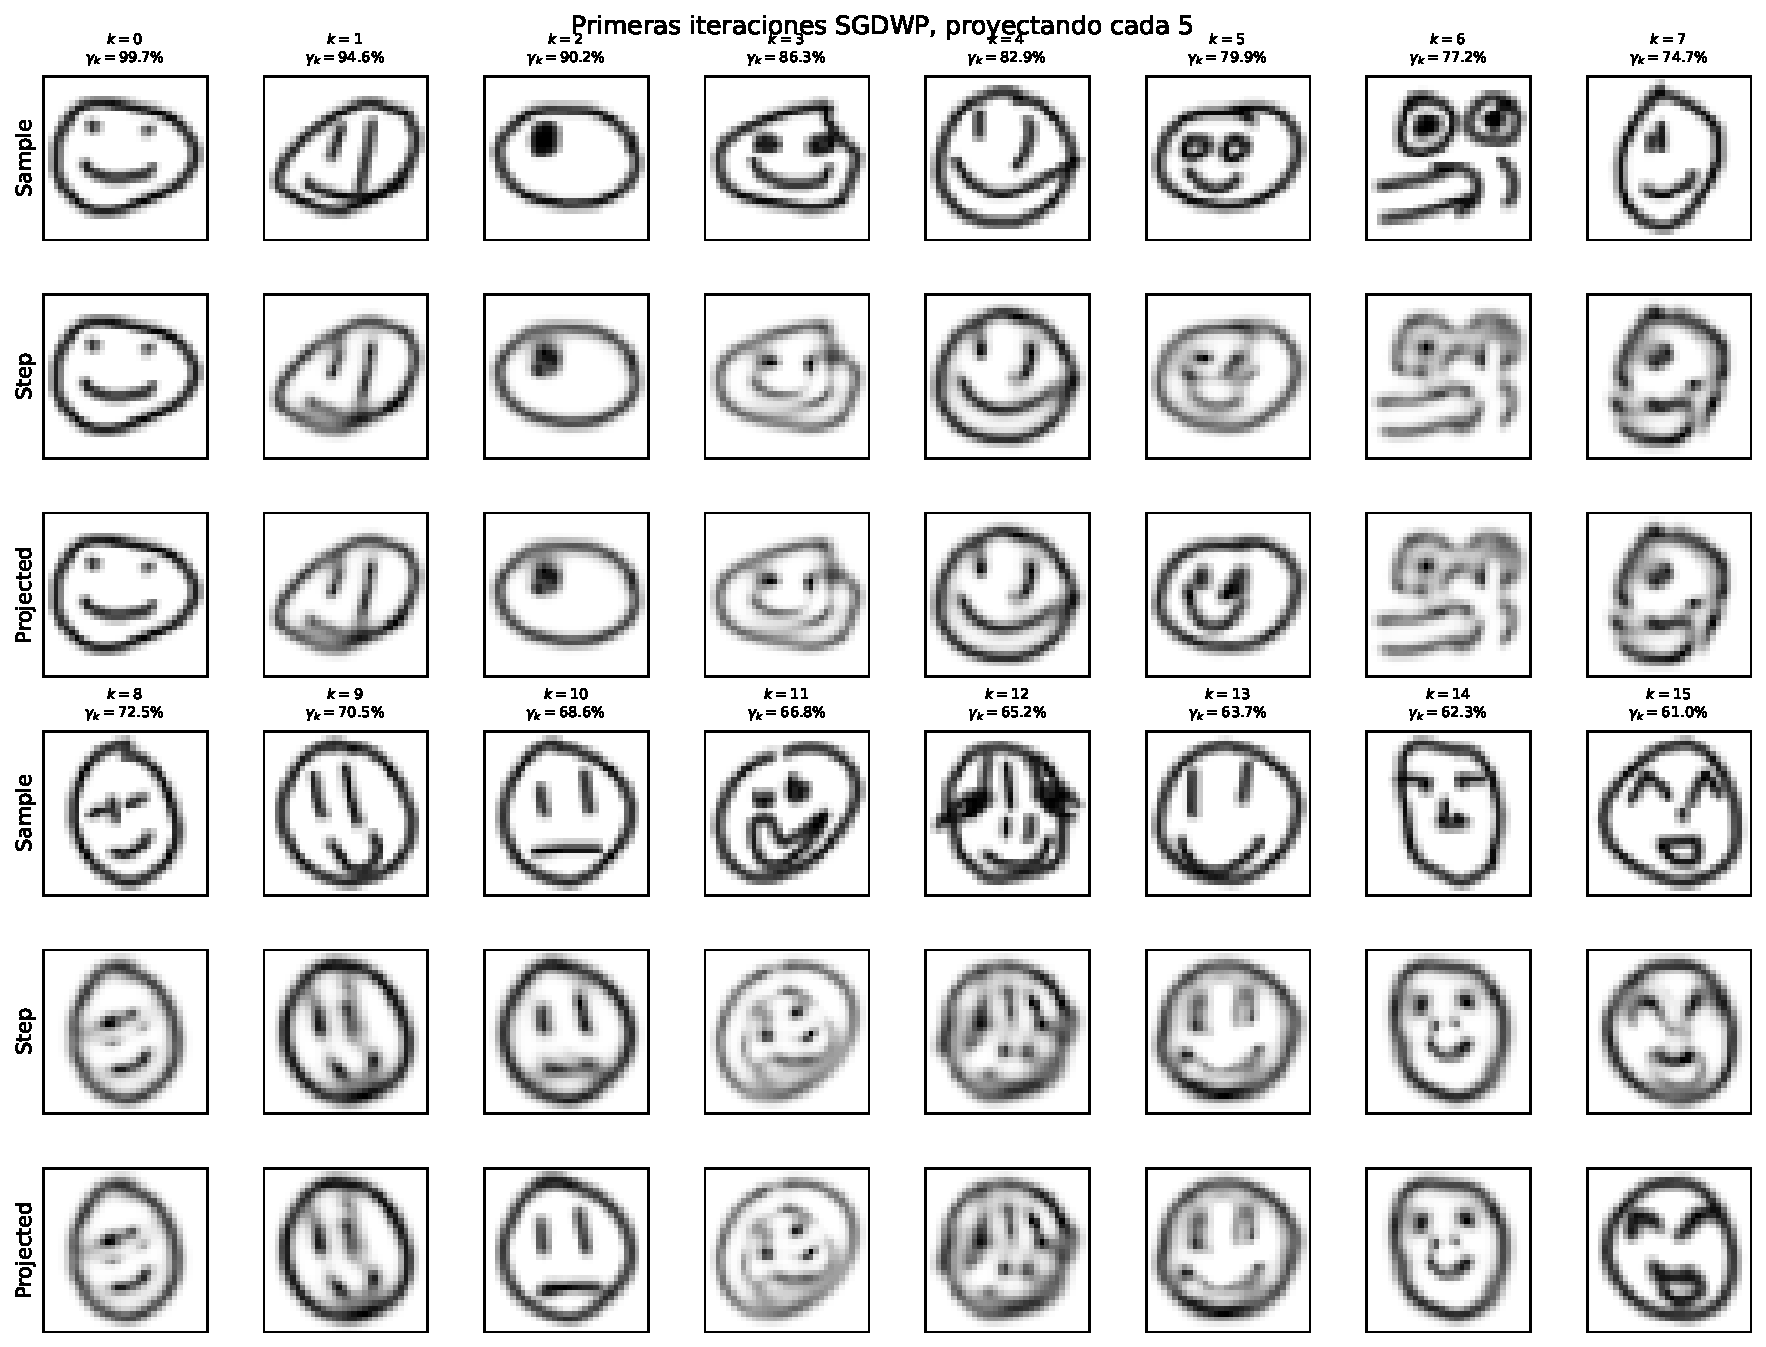
\includegraphics[width=\textwidth]{img/sgdwp-pe-iters/first-iters-pe-05.pdf}
        \caption{Primeras iteraciones del baricentro de la Fig.~\ref{fig:bar-SGDWP-pe-05}}
        \label{fig:first-iters-pe-05}
    \end{subfigure}
    \begin{subfigure}[b]{0.8\textwidth}
        \centering
        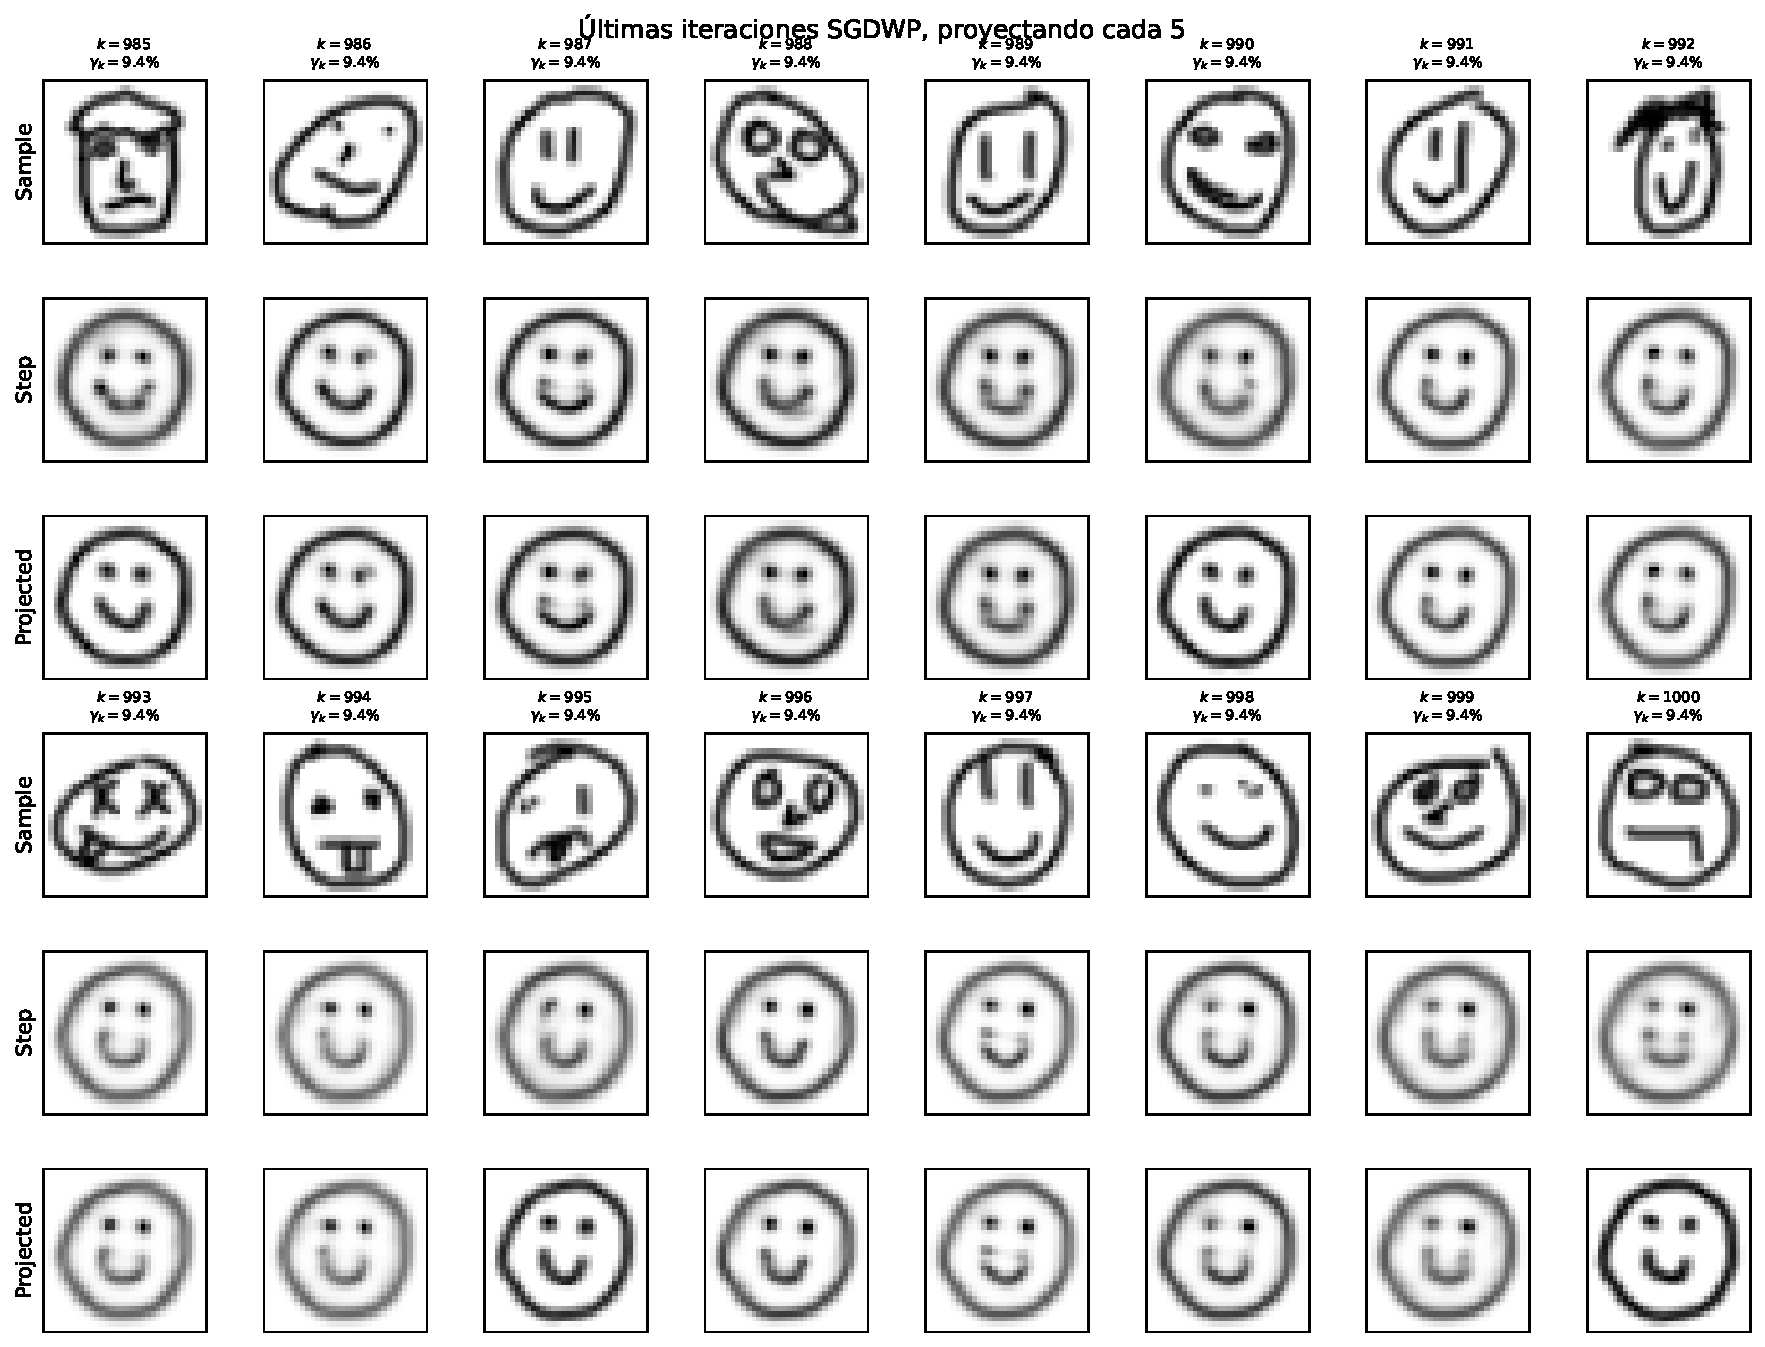
\includegraphics[width=\textwidth]{img/sgdwp-pe-iters/last-iters-pe-05.pdf}
        \caption{Últimas iteraciones del baricentro de la Fig.~\ref{fig:bar-SGDWP-pe-05}}
        \label{fig:last-iters-pe-05}
    \end{subfigure}
    \caption{Iteraciones del cálculo del baricentro de la Fig.~\ref{fig:bar-SGDWP-pe-05}.}
    \label{fig:iters-pe-05}
\end{figure}

\begin{figure}[htbp]
    \centering
    \begin{subfigure}[b]{0.8\textwidth}
        \centering
        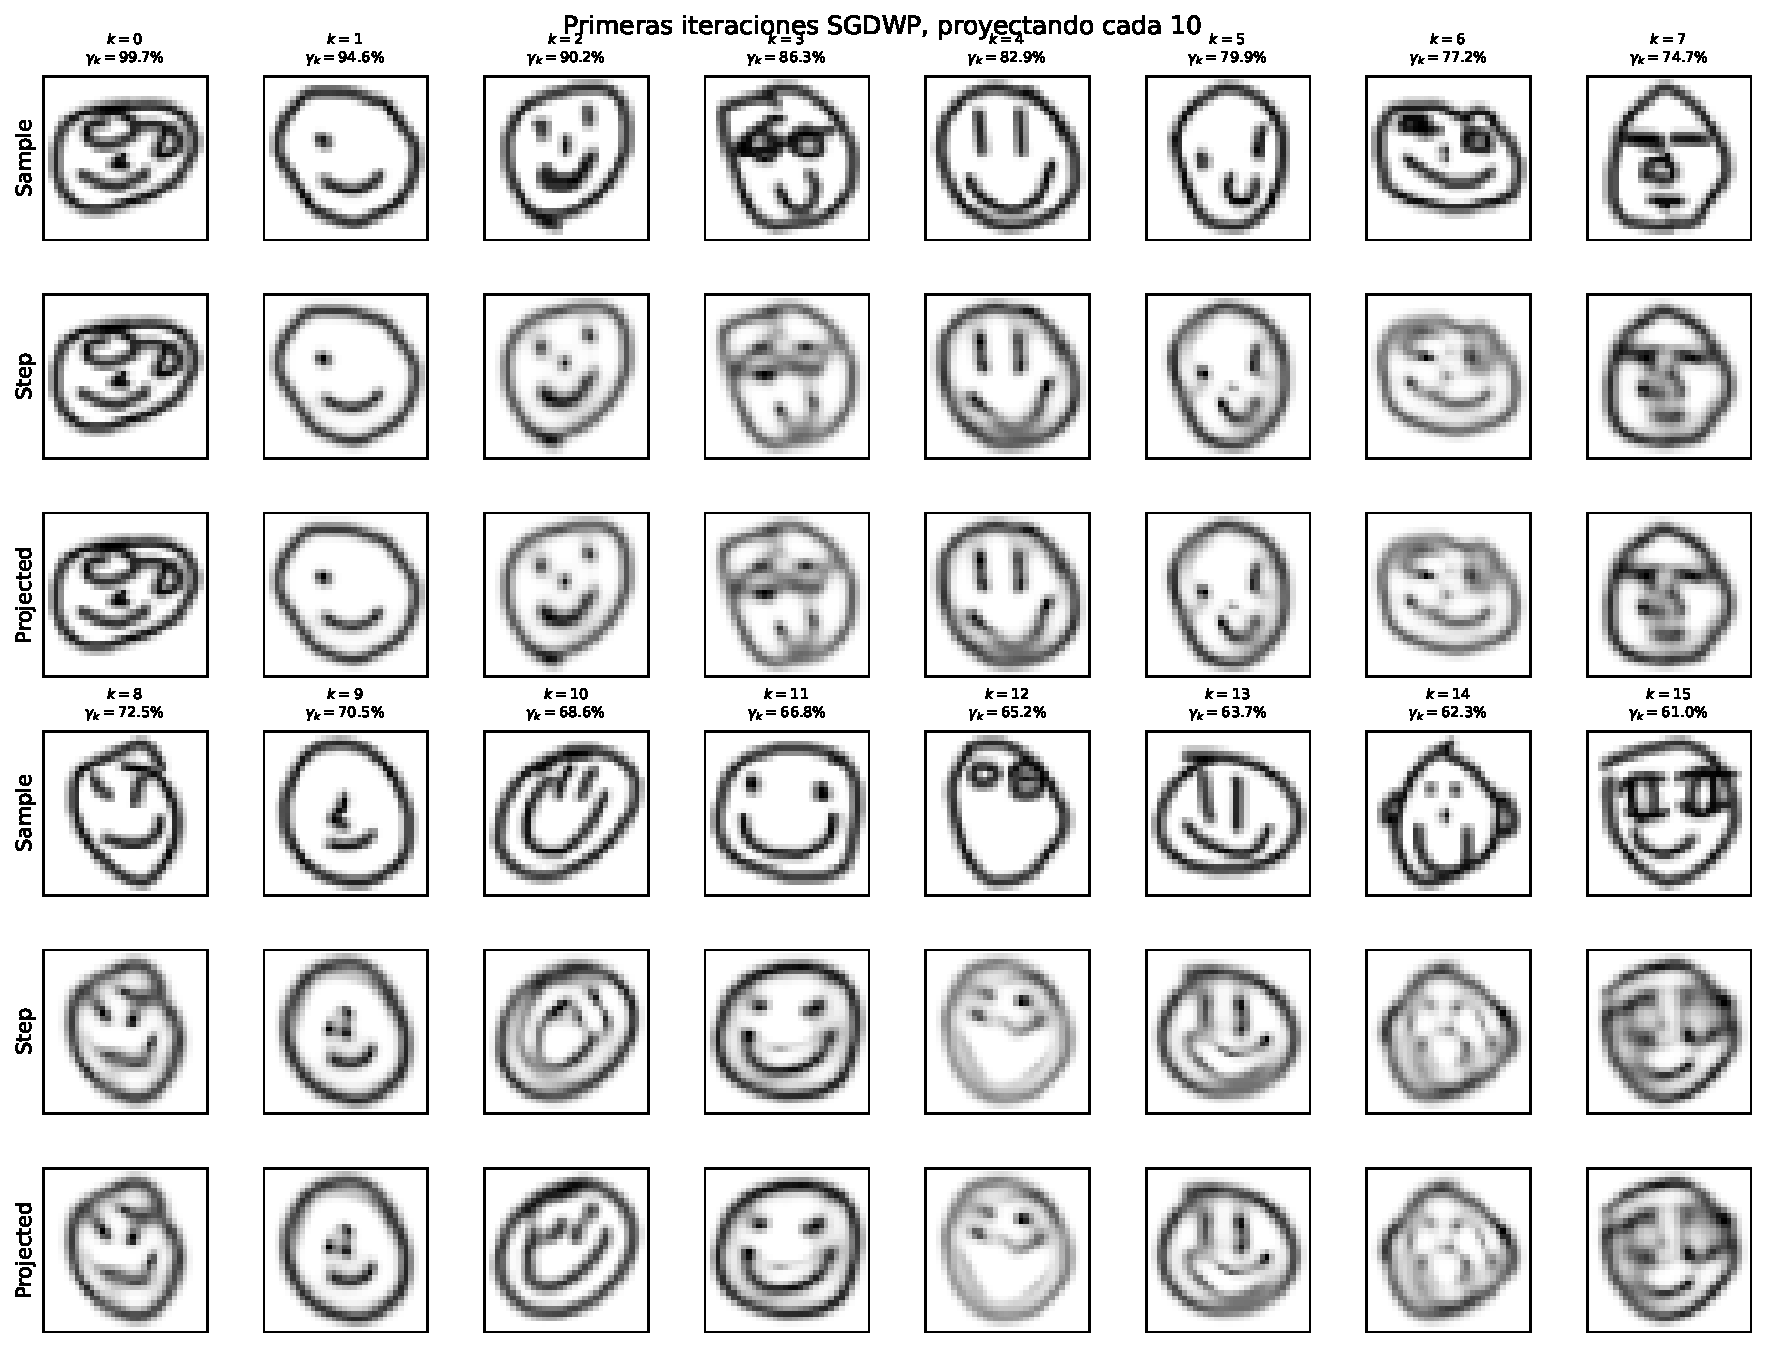
\includegraphics[width=\textwidth]{img/sgdwp-pe-iters/first-iters-pe-10.pdf}
        \caption{Primeras iteraciones del baricentro de la Fig.~\ref{fig:bar-SGDWP-pe-10}}
        \label{fig:first-iters-pe-10}
    \end{subfigure}
    \begin{subfigure}[b]{0.8\textwidth}
        \centering
        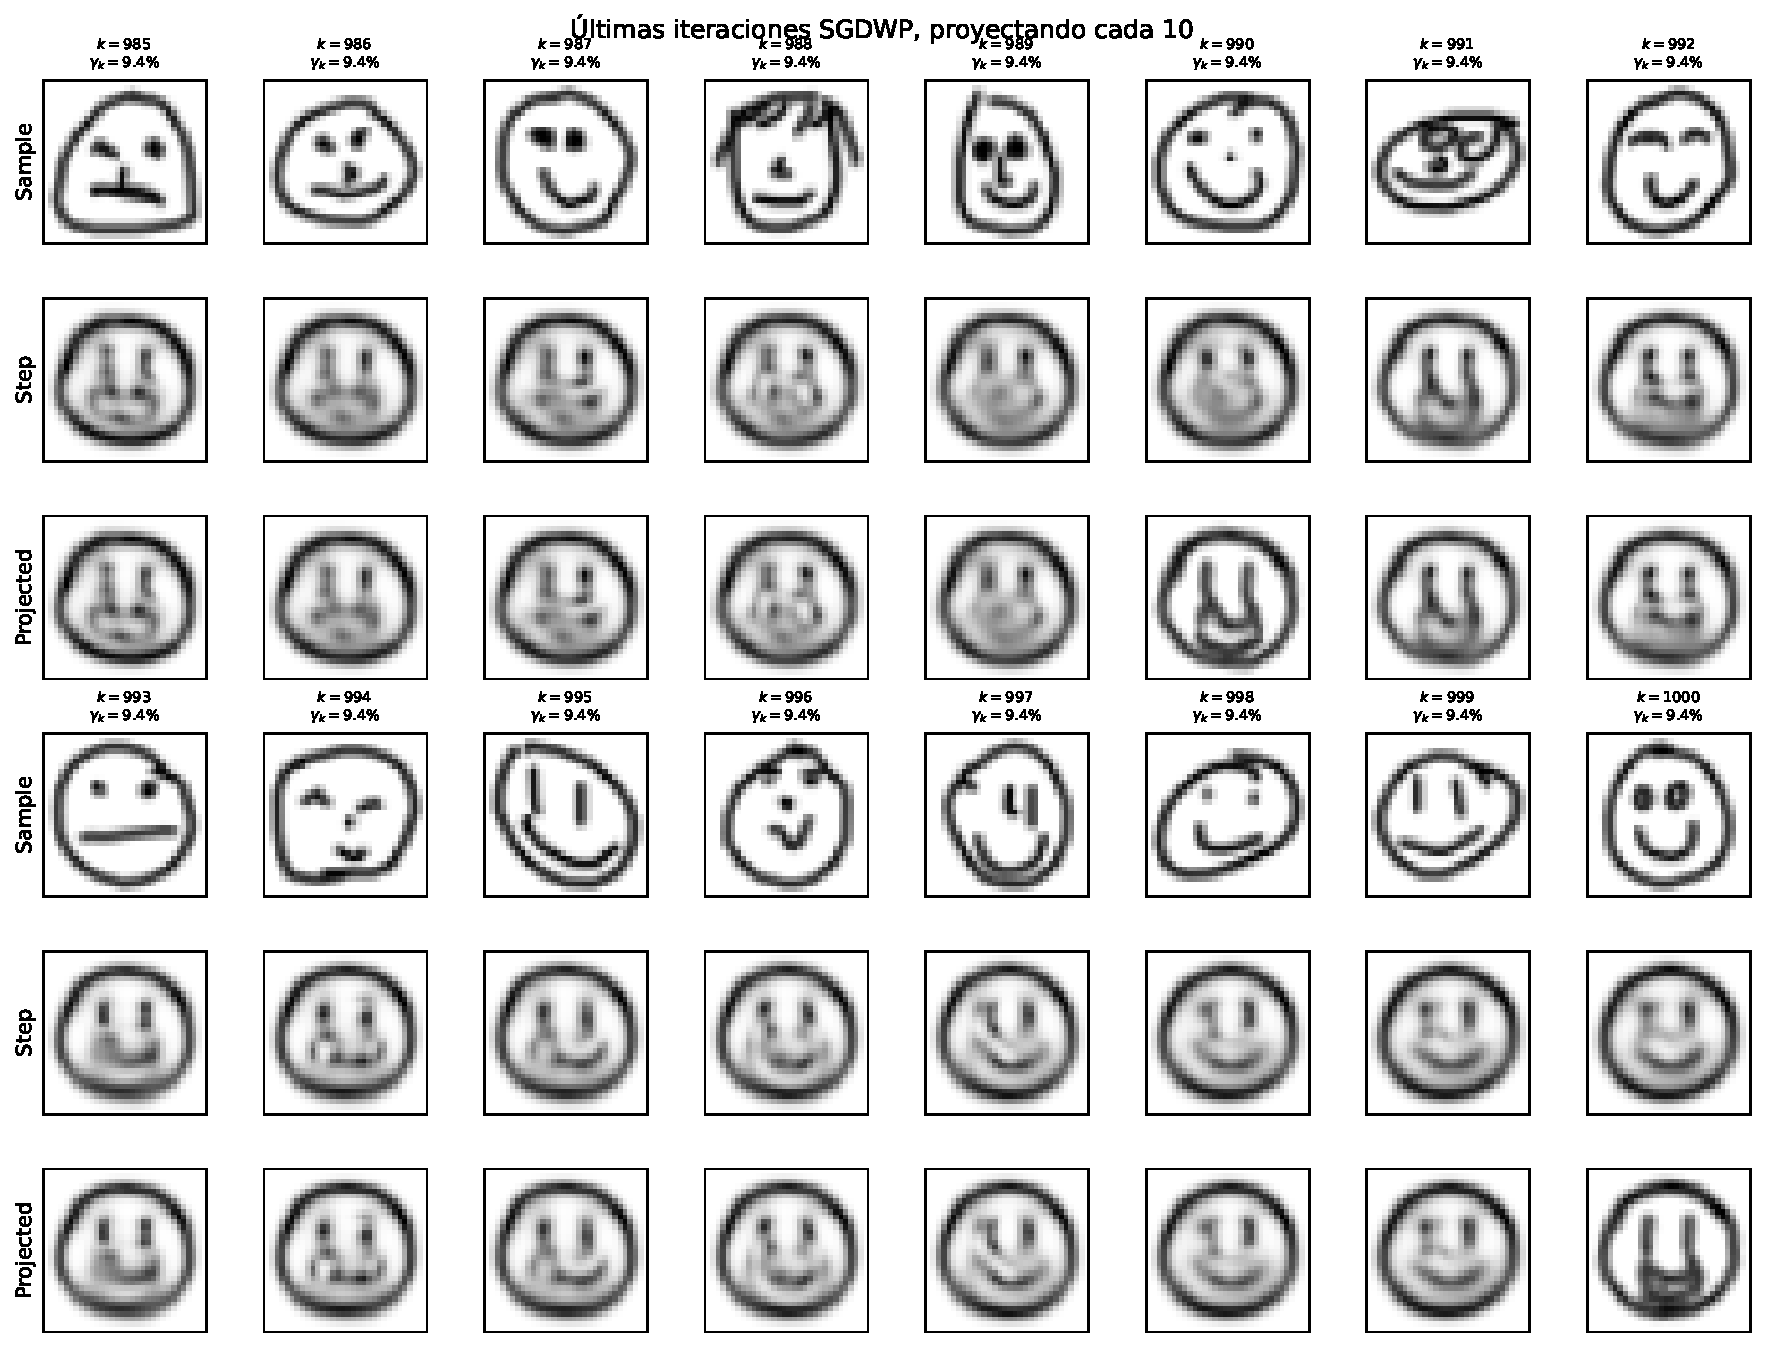
\includegraphics[width=\textwidth]{img/sgdwp-pe-iters/last-iters-pe-10.pdf}
        \caption{Últimas iteraciones del baricentro de la Fig.~\ref{fig:bar-SGDWP-pe-10}}
        \label{fig:last-iters-pe-10}
    \end{subfigure}
    \caption{Iteraciones del cálculo del baricentro de la Fig.~\ref{fig:bar-SGDWP-pe-10}.}
    \label{fig:iters-pe-10}
\end{figure}